% Options for packages loaded elsewhere
\PassOptionsToPackage{unicode}{hyperref}
\PassOptionsToPackage{hyphens}{url}
%
\documentclass[
]{book}
\usepackage{lmodern}
\usepackage{amssymb,amsmath}
\usepackage{ifxetex,ifluatex}
\ifnum 0\ifxetex 1\fi\ifluatex 1\fi=0 % if pdftex
  \usepackage[T1]{fontenc}
  \usepackage[utf8]{inputenc}
  \usepackage{textcomp} % provide euro and other symbols
\else % if luatex or xetex
  \usepackage{unicode-math}
  \defaultfontfeatures{Scale=MatchLowercase}
  \defaultfontfeatures[\rmfamily]{Ligatures=TeX,Scale=1}
\fi
% Use upquote if available, for straight quotes in verbatim environments
\IfFileExists{upquote.sty}{\usepackage{upquote}}{}
\IfFileExists{microtype.sty}{% use microtype if available
  \usepackage[]{microtype}
  \UseMicrotypeSet[protrusion]{basicmath} % disable protrusion for tt fonts
}{}
\makeatletter
\@ifundefined{KOMAClassName}{% if non-KOMA class
  \IfFileExists{parskip.sty}{%
    \usepackage{parskip}
  }{% else
    \setlength{\parindent}{0pt}
    \setlength{\parskip}{6pt plus 2pt minus 1pt}}
}{% if KOMA class
  \KOMAoptions{parskip=half}}
\makeatother
\usepackage{xcolor}
\IfFileExists{xurl.sty}{\usepackage{xurl}}{} % add URL line breaks if available
\IfFileExists{bookmark.sty}{\usepackage{bookmark}}{\usepackage{hyperref}}
\hypersetup{
  pdftitle={MA22004 Course Design Plan},
  pdfauthor={Dr Eric Hall (ehall001@dundee.ac.uk)},
  hidelinks,
  pdfcreator={LaTeX via pandoc}}
\urlstyle{same} % disable monospaced font for URLs
\usepackage{color}
\usepackage{fancyvrb}
\newcommand{\VerbBar}{|}
\newcommand{\VERB}{\Verb[commandchars=\\\{\}]}
\DefineVerbatimEnvironment{Highlighting}{Verbatim}{commandchars=\\\{\}}
% Add ',fontsize=\small' for more characters per line
\usepackage{framed}
\definecolor{shadecolor}{RGB}{248,248,248}
\newenvironment{Shaded}{\begin{snugshade}}{\end{snugshade}}
\newcommand{\AlertTok}[1]{\textcolor[rgb]{0.94,0.16,0.16}{#1}}
\newcommand{\AnnotationTok}[1]{\textcolor[rgb]{0.56,0.35,0.01}{\textbf{\textit{#1}}}}
\newcommand{\AttributeTok}[1]{\textcolor[rgb]{0.77,0.63,0.00}{#1}}
\newcommand{\BaseNTok}[1]{\textcolor[rgb]{0.00,0.00,0.81}{#1}}
\newcommand{\BuiltInTok}[1]{#1}
\newcommand{\CharTok}[1]{\textcolor[rgb]{0.31,0.60,0.02}{#1}}
\newcommand{\CommentTok}[1]{\textcolor[rgb]{0.56,0.35,0.01}{\textit{#1}}}
\newcommand{\CommentVarTok}[1]{\textcolor[rgb]{0.56,0.35,0.01}{\textbf{\textit{#1}}}}
\newcommand{\ConstantTok}[1]{\textcolor[rgb]{0.00,0.00,0.00}{#1}}
\newcommand{\ControlFlowTok}[1]{\textcolor[rgb]{0.13,0.29,0.53}{\textbf{#1}}}
\newcommand{\DataTypeTok}[1]{\textcolor[rgb]{0.13,0.29,0.53}{#1}}
\newcommand{\DecValTok}[1]{\textcolor[rgb]{0.00,0.00,0.81}{#1}}
\newcommand{\DocumentationTok}[1]{\textcolor[rgb]{0.56,0.35,0.01}{\textbf{\textit{#1}}}}
\newcommand{\ErrorTok}[1]{\textcolor[rgb]{0.64,0.00,0.00}{\textbf{#1}}}
\newcommand{\ExtensionTok}[1]{#1}
\newcommand{\FloatTok}[1]{\textcolor[rgb]{0.00,0.00,0.81}{#1}}
\newcommand{\FunctionTok}[1]{\textcolor[rgb]{0.00,0.00,0.00}{#1}}
\newcommand{\ImportTok}[1]{#1}
\newcommand{\InformationTok}[1]{\textcolor[rgb]{0.56,0.35,0.01}{\textbf{\textit{#1}}}}
\newcommand{\KeywordTok}[1]{\textcolor[rgb]{0.13,0.29,0.53}{\textbf{#1}}}
\newcommand{\NormalTok}[1]{#1}
\newcommand{\OperatorTok}[1]{\textcolor[rgb]{0.81,0.36,0.00}{\textbf{#1}}}
\newcommand{\OtherTok}[1]{\textcolor[rgb]{0.56,0.35,0.01}{#1}}
\newcommand{\PreprocessorTok}[1]{\textcolor[rgb]{0.56,0.35,0.01}{\textit{#1}}}
\newcommand{\RegionMarkerTok}[1]{#1}
\newcommand{\SpecialCharTok}[1]{\textcolor[rgb]{0.00,0.00,0.00}{#1}}
\newcommand{\SpecialStringTok}[1]{\textcolor[rgb]{0.31,0.60,0.02}{#1}}
\newcommand{\StringTok}[1]{\textcolor[rgb]{0.31,0.60,0.02}{#1}}
\newcommand{\VariableTok}[1]{\textcolor[rgb]{0.00,0.00,0.00}{#1}}
\newcommand{\VerbatimStringTok}[1]{\textcolor[rgb]{0.31,0.60,0.02}{#1}}
\newcommand{\WarningTok}[1]{\textcolor[rgb]{0.56,0.35,0.01}{\textbf{\textit{#1}}}}
\usepackage{longtable,booktabs}
% Correct order of tables after \paragraph or \subparagraph
\usepackage{etoolbox}
\makeatletter
\patchcmd\longtable{\par}{\if@noskipsec\mbox{}\fi\par}{}{}
\makeatother
% Allow footnotes in longtable head/foot
\IfFileExists{footnotehyper.sty}{\usepackage{footnotehyper}}{\usepackage{footnote}}
\makesavenoteenv{longtable}
\usepackage{graphicx}
\makeatletter
\def\maxwidth{\ifdim\Gin@nat@width>\linewidth\linewidth\else\Gin@nat@width\fi}
\def\maxheight{\ifdim\Gin@nat@height>\textheight\textheight\else\Gin@nat@height\fi}
\makeatother
% Scale images if necessary, so that they will not overflow the page
% margins by default, and it is still possible to overwrite the defaults
% using explicit options in \includegraphics[width, height, ...]{}
\setkeys{Gin}{width=\maxwidth,height=\maxheight,keepaspectratio}
% Set default figure placement to htbp
\makeatletter
\def\fps@figure{htbp}
\makeatother
\setlength{\emergencystretch}{3em} % prevent overfull lines
\providecommand{\tightlist}{%
  \setlength{\itemsep}{0pt}\setlength{\parskip}{0pt}}
\setcounter{secnumdepth}{5}
\usepackage[]{natbib}
\bibliographystyle{plainnat}

\title{MA22004 Course Design Plan}
\author{Dr Eric Hall \href{mailto:ehall001@dundee.ac.uk}{(ehall001@dundee.ac.uk)}}
\date{2020-07-16}

\begin{document}
\maketitle

{
\setcounter{tocdepth}{1}
\tableofcontents
}
\hypertarget{learning}{%
\chapter{Learning}\label{learning}}

\begin{quote}
\emph{Wir shaffen das.}
\end{quote}

\emph{Summary:} runs for 11 weeks (20 SCQF/10 ECTS) approx 200 hours student effort including 55 contact hours.

There will be 1 seminars of one-hour each (\textbf{timetabled, online}), 1 workshop of one-hour (\textbf{timetabled, face-to-face}), and 1 lab of two hours (\textbf{online, asynchronous}). The expectation will be that students access and engage with the lecture notes and curated digital content before participating in the seminar.

\hypertarget{asynchronous-content}{%
\section*{Asynchronous content}\label{asynchronous-content}}
\addcontentsline{toc}{section}{Asynchronous content}

All of this content will be available online.

\begin{description}
\tightlist
\item[Course notes (ACQUIRING)]
\textbf{needs to be prepared} (use of existing hand-written notes with some modificaitons), this content will consist of HTML and PDF notes generated using \texttt{Rmarkdown}.
\item[Interactive computer labs (PRODUCING, PRACTICING)]
\textbf{needs to be prepared} (use of prepared labs with content converted to \texttt{Rmarkdown} and interactive elements added), this content will consist of interactive \texttt{R} computer labs coded using \texttt{learnr} and \texttt{gradethis}. \textbf{Digital \protect\hyperlink{needs}{need}:} RStudio Cloud.
\item[Curated digital content (INQUIRING)]
a collection of digital content for students to explore, e.g., online lectures by \href{https://www.youtube.com/watch?v=a1PtQ67urG4}{David Spiegelhalter}, \href{https://www.youtube.com/watch?v=hVimVzgtD6w}{Hans Rosling}, etc; \href{http://tylervigen.com/spurious-correlations}{spurious correlations}, \href{\%5Bhttps://www.autodeskresearch.com/publications/samestats}{Datasaurus Dozen}, etc. Shared via Blackboard or \href{https://padlet.com/}{padlet}.
\end{description}

\hypertarget{synchronous-content}{%
\section*{Synchronous content}\label{synchronous-content}}
\addcontentsline{toc}{section}{Synchronous content}

This content must be \textbf{timetabled}.

\hypertarget{face-to-face}{%
\subsection*{Face-to-face}\label{face-to-face}}
\addcontentsline{toc}{subsection}{Face-to-face}

\begin{description}
\tightlist
\item[Workshops (PRACTICING, COLLABORATING, DISCUSSING)]
In which students will meet together to work in small groups (5 or 6). The first couple of meetings will involve meeting outdoors, e.g., UoD Botanical Gardens or a park, to collect data (circumference of trees, heights of people, number of people crossing at a busy intersection, etc) that will later be discussed an analyzed. The students will utilized worksheet handouts that are already prepared.
\end{description}

\hypertarget{online}{%
\subsection*{Online}\label{online}}
\addcontentsline{toc}{subsection}{Online}

\begin{description}
\tightlist
\item[Seminars (DISCUSSING, PRODUCING, PRACTICING)]
In which we will have a discussion of the main topics for the week, guided by student polling (using either \href{https://www.mentimeter.com/}{mentimeter} or \href{https://itempool.com/}{itempool}. Periodic quizzes will be given in seminars to assess student attainment. A portion of each seminar will involve a lab presentation given by one of the groups.
\item[Examinations (PRODUCING)]
Midterm and Final examinations will need to be timetabled to lessen the chance of cheating. The Final Examination can also be given during the May diet.
\end{description}

\hypertarget{engagement}{%
\chapter{Engagement}\label{engagement}}

\begin{quote}
The active learning categorization for each teaching task are identified in \protect\hyperlink{learning}{§ Learning}
\end{quote}

There are several points that can be measured to assess engagement, including:

\begin{itemize}
\tightlist
\item
  Students will be presented with a new collection of notes that will roll out weekly using a tool like \href{https://perusall.com/}{perusall} (or possibly Blackboard forums). They will be responsible for posting both questions and responses to the message boards for each new collection of notes.\\
\item
  During seminars, students will be presented with \textbf{polls} to encourage reflection and discussion.
\item
  During seminars, students will take turns giving a lab report \textbf{presentation} with their workshop groups. This will encourage students to challenge each others analysis.
\item
  Students will be expected to hand-in assignments for continuous assessment.
\item
  Students will be expected to sit Midterm examinations. The grades of these examinations will offer opportunities for intervention.
\end{itemize}

\hypertarget{attainment}{%
\chapter{Attainment}\label{attainment}}

\hypertarget{assessment}{%
\chapter{Assessment}\label{assessment}}

The module assessment will be weighted:

\begin{tabular}{l|l}
\hline
Assessment & Weight\\
\hline
Assignments & 20\%\\
\hline
Midterm Exam 1 & 20\%\\
\hline
Midterm Exam 2 & 20\%\\
\hline
Final Exam & 40\%\\
\hline
\end{tabular}

Note: This is a modification from the previous split (60\% degree exam, 20\% two
class tests, and 20\% coursework). As the students will not be given a revision period, the Final Exam will need to be less cumulative in scope and therefore additional weight will be placed on the Midterm Exams.

\hypertarget{examinations}{%
\section*{Examinations}\label{examinations}}
\addcontentsline{toc}{section}{Examinations}

The \textbf{Final Exam} will be a two-hour hand-written exam. Students will be given one additional hour to scan, code, and upload their manuscripts using \href{https://www.gradescope.com/}{gradescope}. This process will be thoroughly discussed and practiced by the students with a dummy exam in advance of a real submission. The Final Exam will either be given in the last week of term (week 11) or during the May exam diet.

The \textbf{Midterm Exams} will either be hand-written or computer-assessed and will be one-hour in scope instead of two. These will likely be held in week 4 and week 8.

\hypertarget{assignments}{%
\section*{Assignments}\label{assignments}}
\addcontentsline{toc}{section}{Assignments}

The assessed courwork will include 6 lab reports and 1 lab report presentation (group work).

\hypertarget{needs}{%
\chapter{NEEDS}\label{needs}}

\hypertarget{digital-needs}{%
\section*{Digital needs}\label{digital-needs}}
\addcontentsline{toc}{section}{Digital needs}

\begin{enumerate}
\def\labelenumi{\arabic{enumi}.}
\tightlist
\item
  bringing computer lab into cloud: semester subsription to \href{https://rstudio.cloud/}{RStudio Cloud}\footnote{A better long-term solution would be to run \texttt{RStudio\ Server\ Pro} and \texttt{RStudio\ Connect} on in-house server running, licenses are available for \href{https://rstudio.com/pricing/academic-pricing/}{free} for teaching purposes.} (approx. 1000 USD)
\item
  polling: \href{https://www.mentimeter.com/}{mentimeter} or \href{https://itempool.com/}{itempool}
\end{enumerate}

\hypertarget{hardware-needs}{%
\section*{Hardware needs}\label{hardware-needs}}
\addcontentsline{toc}{section}{Hardware needs}

\begin{enumerate}
\def\labelenumi{\arabic{enumi}.}
\tightlist
\item
  Better microphone
\item
  Tablet with stylus
\end{enumerate}

\hypertarget{rmarkdown-example}{%
\chapter*{Rmarkdown Example}\label{rmarkdown-example}}
\addcontentsline{toc}{chapter}{Rmarkdown Example}

\hypertarget{math}{%
\section*{Math}\label{math}}
\addcontentsline{toc}{section}{Math}

Here is an example page containing math markdown.

\begin{Shaded}
\begin{Highlighting}[]
\NormalTok{We can use inline math, }\SpecialStringTok{$f\_X$}\NormalTok{, }\SpecialStringTok{$f\_Y$}\NormalTok{, and }\SpecialStringTok{$f\_\{X,Y\}$}\NormalTok{, as well as display math, }
\SpecialStringTok{\textbackslash{}[}
\SpecialStringTok{  I(X;Y)}
\SpecialStringTok{  = }\SpecialCharTok{\textbackslash{}iint}\SpecialStringTok{\_\{}\SpecialCharTok{\textbackslash{}mathcal}\SpecialStringTok{\{X\} }\SpecialCharTok{\textbackslash{}otimes}\SpecialStringTok{ }\SpecialCharTok{\textbackslash{}mathcal}\SpecialStringTok{\{Y\}\}}
\SpecialStringTok{  }\SpecialCharTok{\textbackslash{}log\textbackslash{}left}\SpecialStringTok{( }\SpecialCharTok{\textbackslash{}frac}\SpecialStringTok{\{f\_\{X,Y\}(x,y)\}\{f\_\{X\}(x)f\_\{Y\}(y)\} }\SpecialCharTok{\textbackslash{}right}\SpecialStringTok{)}
\SpecialStringTok{  f\_\{X,Y\}(x,y) }\SpecialCharTok{\textbackslash{}mathrm}\SpecialStringTok{\{d\}y }\SpecialCharTok{\textbackslash{}mathrm}\SpecialStringTok{\{d\}x}\SpecialCharTok{\textbackslash{},}\SpecialStringTok{.}
\SpecialStringTok{\textbackslash{}]}
\end{Highlighting}
\end{Shaded}

to generate:

We can use inline math, \(f_X\), \(f_Y\), and \(f_{X,Y}\), as well as display math,
\[
  I(X;Y)
  = \iint_{\mathcal{X} \otimes \mathcal{Y}}
  \log\left( \frac{f_{X,Y}(x,y)}{f_{X}(x)f_{Y}(y)} \right)
  f_{X,Y}(x,y) \mathrm{d}y \mathrm{d}x\,.
\]

\hypertarget{plots}{%
\section*{Plots}\label{plots}}
\addcontentsline{toc}{section}{Plots}

\begin{Shaded}
\begin{Highlighting}[]
\NormalTok{x \textless{}{-}}\StringTok{ }\KeywordTok{seq}\NormalTok{(}\OperatorTok{{-}}\DecValTok{8}\NormalTok{, }\DecValTok{8}\NormalTok{, }\DataTypeTok{length=}\DecValTok{1000}\NormalTok{)}
\NormalTok{y0 \textless{}{-}}\StringTok{ }\KeywordTok{dnorm}\NormalTok{(x, }\DecValTok{{-}2}\NormalTok{, }\DecValTok{1}\NormalTok{)}
\NormalTok{y1 \textless{}{-}}\StringTok{ }\KeywordTok{dnorm}\NormalTok{(x, }\DecValTok{2}\NormalTok{, }\DecValTok{1}\NormalTok{)}
\NormalTok{df \textless{}{-}}\StringTok{ }\KeywordTok{tibble}\NormalTok{(x, y0, y1)}
\NormalTok{df \textless{}{-}}\StringTok{ }\KeywordTok{melt}\NormalTok{(df, }\DataTypeTok{id.var =} \StringTok{"x"}\NormalTok{, }\DataTypeTok{value.name =} \StringTok{"y"}\NormalTok{)}

\KeywordTok{ggplot}\NormalTok{(}\DataTypeTok{data =}\NormalTok{ df, }\KeywordTok{aes}\NormalTok{(}\DataTypeTok{x =}\NormalTok{ x, }\DataTypeTok{color =}\NormalTok{ variable)) }\OperatorTok{+}\StringTok{ }\KeywordTok{geom\_line}\NormalTok{(}\KeywordTok{aes}\NormalTok{(}\DataTypeTok{y=}\NormalTok{y)) }
\end{Highlighting}
\end{Shaded}

\begin{figure}
\centering
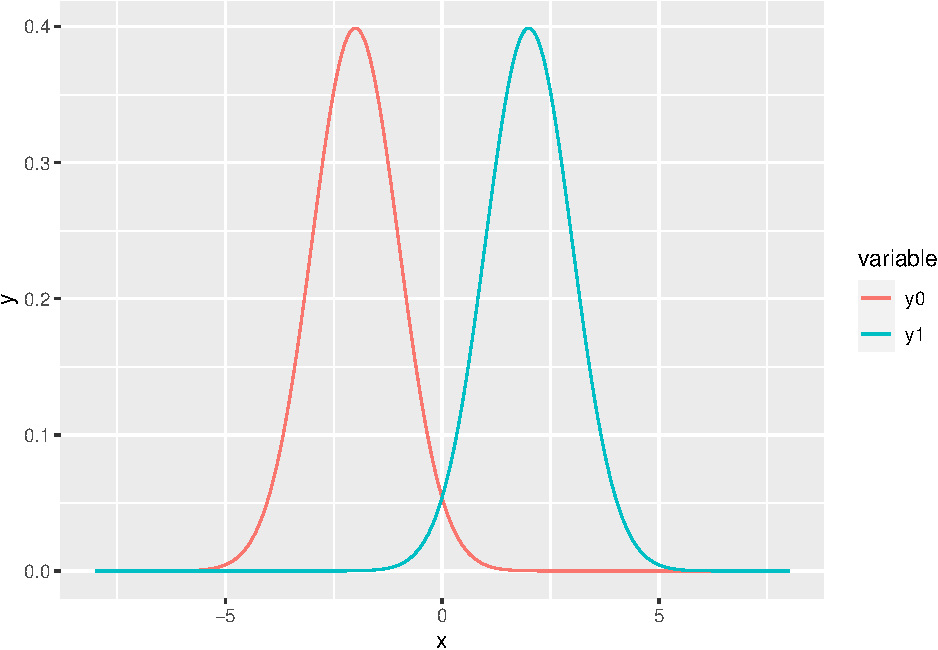
\includegraphics{design-notes_files/figure-latex/normals-same-var-1.pdf}
\caption{\label{fig:normals-same-var}Two normal variates with different means and same variance. Note this figure is a scalable vector graphic --- from what I understand, this is better from an accessbility standpoint.}
\end{figure}

The figure with caption caption is created by typing the code directly into the markdown document:

\begin{verbatim}
```{r normals-same-var, echo=TRUE, fig.cap="Two normal variates with different means and same variance. Note this figure is a scalable vector graphic --- from what I understand, this is better from an accessbility standpoint."}
  x <- seq(-8, 8, length=1000)
  y0 <- dnorm(x, -2, 1)
  y1 <- dnorm(x, 2, 1)
  df <- tibble(x, y0, y1)
  df <- melt(df, id.var = "x", value.name = "y")
  ggplot(data = df, aes(x = x, color = variable)) + geom_line(aes(y=y)) 
```
\end{verbatim}

\end{document}
